\chapter{Introduction}\label{chap:1}

The main objective of this final degree project is to continue the development of an SDN-based DMM mobility solution project under the CROWD EU FP7 scheme\footnote{\url{http://www.ict-crowd.eu/}}, by means of expanding and improving the functionalities. Some of the functionalities included in the project are: LTE connectivity emulation, video streaming capabilities with on-going mobility between access points, on-demand infrastructure for resource management and multi-mobile-node capability.\\

This project encompasses the combination of Software-Defined Networking (SDN) and Distributed Mobility Management (DMM) as a networking solution to the mobility problems in extremely dense wireless networks.\\

SDN is an approach to networking that involves the separation of the control plane from the data forwarding plane, resulting in the capacity to manage network behaviour dynamically. This is achieved through the abstraction of the forwarding plane using standardized interfaces \cite{rfc_7426}. A more detailed description can be found in Chapter [insert reference] of State of the Art.\\

DMM suggests a distributed network structure compared to a centralized structure to defeat the limitations of existing network protcols that use centrally deployed mobility anchors such as Mobile IP \cite{rfc_6275}. A broader view of this approach is located in Chapter \ref{sec:chap2_dmm} of State of the Art.\\

Together SDN and DMM will deal with the problems standardized mobility protocols will face in ultra dense wireless networks such as inefficiency, bottle necks, scalibility and unreliability.

\begin{center}
\begin{figure}[h!]
  \centering
    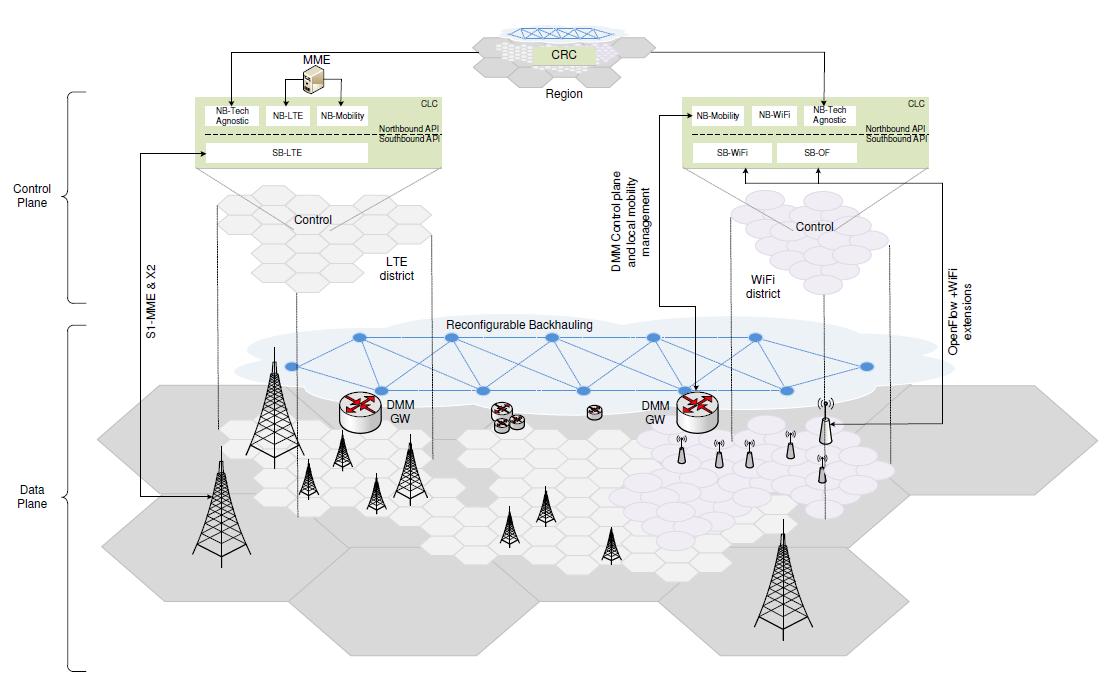
\includegraphics[scale=0.5]{./images/crowd_arch}
	\caption{CROWD Architecture}
	\label{crowd_arch-fig}
\end{figure}
\end{center}

For this project, we started with an implementation of the CROWD project scenario. In this implementation, there are two districts, both managed by a regional controller called CROWD Regional Controller. Under the CROWD Regional Controller, each district is locally managed by a CROWD Local Controller. One of the pilars of this project is LTE emulation integration combining ns3 and NI PXI systems, which is important to have a complete WLAN/RAN architecture.\\

In order to test the performance of this system, we conduct a series of experiments.














